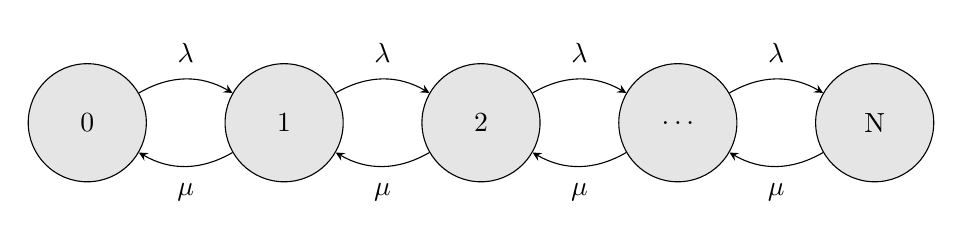
\begin{tikzpicture}[>=stealth, node distance=2.5cm,every node/.style={circle}]
    % Nodes without circles
    \node (0) [draw, fill=gray!20, minimum size=15mm] {0};
    \node (1) [right of=0, draw, fill=gray!20, minimum size=15mm] {1};
    \node (2) [right of=1, draw, fill=gray!20, minimum size=15mm] {2};
    \node (3) [right of=2, draw, fill=gray!20, minimum size=15mm] {$\dots$};
    \node (N) [right of=3, draw, fill=gray!20, minimum size=15mm] {N};

    % Edges with transition rates
    \draw[->, bend left] (0) to node[above] {$\lambda$} (1);
    \draw[->, bend left] (1) to node[above] {$\lambda$} (2);
    \draw[->, bend left] (2) to node[above] {$\lambda$} (3);
    \draw[->, bend left] (3) to node[above] {$\lambda$} (N);

    \draw[->, bend left] (1) to node[below] {$\mu$} (0);
    \draw[->, bend left] (2) to node[below] {$\mu$} (1);
    \draw[->, bend left] (3) to node[below] {$\mu$} (2);
    \draw[->, bend left] (N) to node[below] {$\mu$} (3);

\end{tikzpicture}